% -----------------------------------------------
% Template for ISMIR Papers
% 2017 version, based on previous ISMIR templates

% Requirements :
% * 6+n page length maximum
% * 4MB maximum file size
% * Copyright note must appear in the bottom left corner of first page
% * Clearer statement about citing own work in anonymized submission
% (see conference website for additional details)
% -----------------------------------------------

\documentclass{article}
\usepackage{ismir,amsmath,cite,url}
\usepackage{amsfonts}
\usepackage{graphicx}
\usepackage{color}
\usepackage{microtype}
\usepackage{units}
\usepackage{paralist}


% Title.
% ------
\title{Automatic Sample Detection in Polyphonic Music}

% Note: Please do NOT use \thanks or a \footnote in any of the author markup

% Single address
% To use with only one author or several with the same address
% ---------------
%\oneauthor
% {Names should be omitted for double-blind reviewing}
% {Affiliations should be omitted for double-blind reviewing}

% Two addresses
% --------------
%\twoauthors
%  {First author} {School \\ Department}
%  {Second author} {Company \\ Address}

%% To make customize author list in Creative Common license, uncomment and customize the next line
%  \def\authorname{First Author, Second Author}


% Three addresses
% --------------
\threeauthors
  {First Author} {Affiliation1 \\ {\tt author1@ismir.edu}}
  {Second Author} {\bf Retain these fake authors in\\\bf submission to preserve the formatting}
  {Third Author} {Affiliation3 \\ {\tt author3@ismir.edu}}

%% To make customize author list in Creative Common license, uncomment and customize the next line
%  \def\authorname{First Author, Second Author, Third Author}

% Four or more addresses
% OR alternative format for large number of co-authors
% ------------
%\multauthor
%{First author$^1$ \hspace{1cm} Second author$^1$ \hspace{1cm} Third author$^2$} { \bfseries{Fourth author$^3$ \hspace{1cm} Fifth author$^2$ \hspace{1cm} Sixth author$^1$}\\
%  $^1$ Department of Computer Science, University , Country\\
%$^2$ International Laboratories, City, Country\\
%$^3$  Company, Address\\
%{\tt\small CorrespondenceAuthor@ismir.edu, PossibleOtherAuthor@ismir.edu}
%}
%\def\authorname{First author, Second author, Third author, Fourth author, Fifth author, Sixth author}


\sloppy % please retain sloppy command for improved formatting

\begin{document}

%
\maketitle
%
\begin{abstract}
The term `sampling' refers to the usage of snippets or loops from existing songs or sample libraries in new songs, mashups, or other music productions. The ability to automatically detect sampling in music is, for instance, beneficial for studies tracking artist influences geographically and temporally. We present a method based on Dynamic Time Warping (DTW) and Non-negative Matrix Factorization (NMF) for the automatic detection of a sample in a set of query songs. The method comprises of two processing steps: first, the DTW alignment path between activations of the query song and reference sample is computed. Second, features are extracted from this path and used to train a Random Forest classifier to detect the presence of the sample. The method is able to identify samples that are pitch-shifted and/or time-stretched. We evaluate this method for sample detection against a new publicly available dataset of real-world sample and song pairs.
\end{abstract}
%
\section{Introduction}
\label{sec:intro}

Sampling is, in the context of music composition and production, the concept of reusing pre-existing digital recordings in new compositions in a way that it fits in the musical context. In digital sampling, an artist records a segment of a song or sound that they wish to sample, may or may not modify it, and then reuses it (and possibly other samples) by incorporating it into a new composition \cite{katz_capturing_2004}. Sampling of audio has become popular in mainstream pop, hip-hop, and rap music. 

A sample detection system enables a musicological study of the influence of older artists over newer generation artists by observing sampling patterns over the years and geographically.
%It has also gained attention from legal issues in the practice of digital sampling. Section \ref{Motivation} of this paper will discuss the motivation behind research in sample detection. 
%
Another possible use case of a sample detection system could be to detect plagiarism or copyright infringement. Sampling is legally controversial and determining fair use is largely left to the courthouse. A system that gives an objective measure of the likelihood of a sample being present in an audio file could add weight to either party's argument in a lawsuit.

The algorithm discussed in this paper focuses on solving the problem of detecting the presence of a given sample in a set of songs as well as its time location in the song.

% Although sampling is popular as a musical tool, it has not been subject to much research in the domain of Music Information Retrieval. A few works focusing on sampling shall be discussed in Section \ref{related}. The sections that follow will focus mainly on the work that has been done in this paper, discussing the algorithm, the evaluation, and an outline for future work possible.
%
\section{Related Work}
\label{related}
The task of sample detection has been addressed in only few previous works. However, there are several parallels that may be drawn from other areas of research that are relevant to sample detection such as cover song detection, audio fingerprinting and remix recognition. \tabref{comparison} summarizes the main differences of audio fingerprinting, cover song detection, and sample detection systems. {\color{red}Would it look better to flip the table and put it into one column?}

\begin{table*}[!ht]
\centering
\label{comparison}
\begin{tabular}{|c|c|c|c|}
\hline
\multicolumn{1}{|l|}{}        & \textbf{Audio Fingerprinting} & \textbf{Cover Song Detection} & \textbf{Sample Detection}\\ \hline
\begin{tabular}[c]{@{}c@{}}Similarity of query \\ to reference\end{tabular} & \begin{tabular}[c]{@{}c@{}}Exact audio (degraded) \\ is detected\end{tabular} & \begin{tabular}[c]{@{}c@{}}Cover is not exactly the same \\ audio as the reference\end{tabular}                                 & \begin{tabular}[c]{@{}c@{}}Exact sample is present, \\  but possibly modified \end{tabular}                  \\ \hline
\begin{tabular}[c]{@{}c@{}}Addition of extra \\ audio tracks\end{tabular}   & \begin{tabular}[c]{@{}c@{}}Only query audio is \\ present\end{tabular}         & \begin{tabular}[c]{@{}c@{}}Cover contains modifications \\  (structural, instrumental, \ldots) \end{tabular} & \begin{tabular}[c]{@{}c@{}}Sample is present in a mixture \\ of many other audio tracks \end{tabular} \\ \hline
\end{tabular}
\caption{Comparison Table of Related Work}
\end{table*}

\subsection{Audio Fingerprinting}

Audio fingerprinting refers to the method of extracting content-based signatures from audio \cite{cano2005review}. {\color{red}more references needed?} It is most commonly used in content-based music identification systems like Shazam.\footnote{https://www.shazam.com \color{red}{add access date to all links}}
Van Balen proposed the use audio fingerprinting for sample detection \cite{van2011automatic}, using a popular fingerprinting by Wang \cite{wang2003industrial} in an implementation by Ellis \cite{ellisfinger}. 
% The implementation was adapted to this task by: 
% \begin{enumerate*}
% \item Enabling the system to handle longer audio queries.
% \item Optimizing the parameters for landmark matching.
% \end{enumerate*}

While fingerprinting systems that are robust against attacks such as pitch shifting or time stretching seem to be a good choice for sample detection, a sample is usually only one of many components in a mixture of audio sources. Audio fingerprinting algorithms are designed to detect the exact recording in the presence of noise but can't perform well when the audio is mixed and masked by other audio signals.

\subsection{Cover Song Detection}
Cover song detection is the task of recognizing whether a given reference track has a cover song in a set of test tracks\cite{Ellis2007Cover,serracover,bertin2011large}.
Covers may, for example, be transposed and may vary in tempo from the original song. Dynamic Time Warping (DTW) \cite{berndt1994using} {\color{red}is this the right reference here?} is often used to make these systems tempo invariant. The difference to sample detection lies in the fact that covers are renditions of a musical piece, while samples are snippets of audio which are usually a part of the mix overlaid with multiple other instruments and sounds unrelated to the sample.
%
The evaluation, however, is highly similar. Both have a test/reference pair which is then categorized as a positive or negative match with a confidence measure. {\color{red}add references here}

\subsection{Remix Recognition}
Remix recognition aims at identifying... {\color{red}could you double check this whole paragraph? Your description does not seem to be in line with their abstract. Also, if you have only two authors, you can't use et al. --- that would be plural}
Work done in remix recognition by Casey and Slaney \cite{caseyRemix} draws inspiration from a method for web crawling called `shingling' which utilizes a stream of text position-based features to detect if a document has already been crawled before. In their work, they compute low-level audio features such as pitch-class profiles and Log-Frequency Cepstral Coefficients (LFCCs) using 0.1 second frames. They concatenate these feature vectors into 4 second 'shingles' and model the distribution of pair-wise distances between shingles from remixes and shingles that aren't from remixes. A nearest neighbor classifier is used to identify which distribution a query 'shingle' belongs to. In the context of sample detection, such a system would not work due to the fact that this method relies on long-term similarity between the query and the reference, however, a sample may be short and one-shot.
%They snip an audio track into 4 second `shingles' and search in a set of similarly snipped test tracks using popular low-level audio features such as MFCCs and pitch-class profiles. In sample detection, such a system wouldn't work because the features would capture information of the whole mix instead of just the sample.

\subsection{Sample detection with Non-negative Matrix Factorization}
%
Dittmar et al.\ listed sampling as one or three kinds of plagiarism in music \cite{dittmar2012audio}. They propose to make use of Non-negative Matrix Factorization (NMF) to learn the spectral templates from the sample and detect the presence of these templates in the suspect audio. Correlating the activations from the sample and the song the gives the likelihood of plagiarism.
%
While the authors provide a general outline of a sample detection system, they neither offer a detailed algorithmic description nor a formal evaluation of their proposed system. It appears that sample detection as a task in music information retrieval has not yet been well defined in terms of evaluation methodology or metrics. Up to now, datasets related to sampling are non-existent or proprietary.


\section{Method}
\label{algo}

\begin{figure}[!ht]
\centering
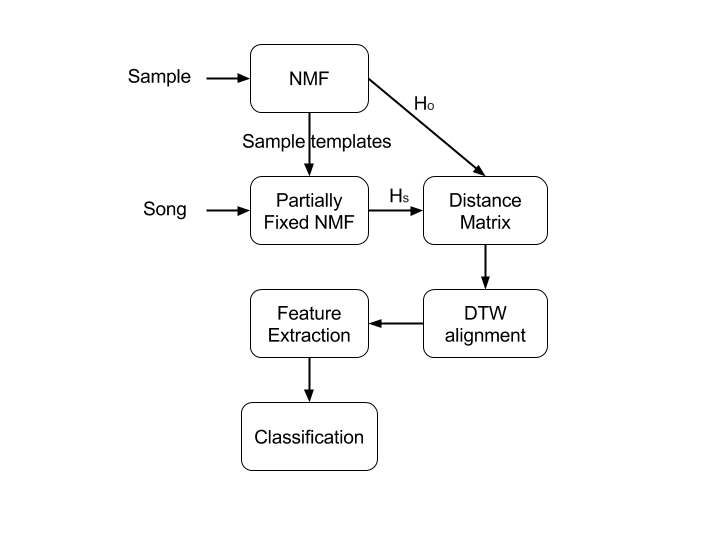
\includegraphics[width=\linewidth]{block_diagram.png}
\caption{Block diagram showing the flow of the algorithm}
\label{fig_block}
\end{figure}

The algorithm presented in this paper is inspired by the work of Dittmar et al.~\cite{dittmar2012audio}. Since the task of sample detection is similar to a source identification problem where the sample is one of the sources present in the mix, an NMF-based approach is fitting due to its prevalence in source separation tasks \cite{virtanen2007monaural}.{\color{red}add more references here} The block diagram in \figref{fig_block} shows the processing steps of the algorithm.

\subsection{Non-Negative Matrix Factorization}
NMF is a widely popular algorithm in unsupervised learning with applications in recommendation systems\cite{koren2009matrix} and signal processing\cite{lee1999learning}{\color{red}why these two references? It seems random}. NMF factorizes a signal $V \in \mathbb{R}^{M\times N}$ into a template matrix $W \in \mathbb{R}^{M\times K}$ and an activation matrix $H \in \mathbb{R}^{K\times N}$:
\[ V \approx W\cdot H.\]
If $V$ is the magnitude spectrogram with $M$ frequency bins and $N$ blocks, $W$ contains the $K$ spectral or harmonic component templates in $V$ while $H$ contains temporal information about each corresponding spectral components in the template matrix \cite{smaragdis2003non}.

In a pre-processing step, both the original sample and the query song are RMS-normalized, downmixed, and downsampled to \unit[22.05]{kHz}; then, their magnitude spectrogram is computed (block size: 4096, hop size: 1024 samples). %Similarly, we preprocess and compute the magnitude spectrogram of the song, which may or may not contain the sample.
Using NMF, the sample spectrogram will be factorized into $K$ templates $W_\mathrm{o}$ and the activation matrix $H_\mathrm{o}$. A sample, used in a song, may be thought of as one source in a mixture of multiple sources in the query song. 
The factorization of the query song will then be performed using partially fixed NMF \cite{wu_drum_2015,wu2015drum}. In this case, the template matrix $W$ consists of a fixed, not updated, part containing the extracted templates $W_\mathrm{o}$ and a randomly initialized part $W_\mathrm{m}$ with $L$ templates that is iteratively learned and represents what we refer to as the mixture templates. The dimension of the complete template matrix is thus $M\times (K+L)$. All activations are iteratively updated as well.

\subsubsection{NMF Rank Selection}
\label{nmfrank}
The rank $K$ of the sample spectrogram has to be chosen based on how many spectral templates need to be used to approximate the specific sample. Similarly, while doing the partially fixed NMF, the rank $L$ for approximating the templates representing the remaining mixture in the song has to be selected in a way that minimizes the impact on the fixed sample template activations in order to robustly detect the sample.

Different songs will usually require different ranks for accurately approximating and factorizing their magnitude spectrograms with a low reconstruction error. In the current algorithm, however, fixed ranks are chosen: $K=10$ and $L=20$. The rationale behind this is that for this task a perfect reconstruction is not required and that the DTW should be robust enough to detect the sample and regardless of whether the templates are able to combine linearly to accurately reconstruct the original spectrogram. If the sample is used in a song, the same fixed templates should produce a roughly similar set of activations regardless of the harmonic rank. 

A possible extension could be to analyze the audio separately as a pre-processing step to obtain an approximate `complexity' of the audio and adapt the ranks $K$ and $L$ based on the complexity of signals to be modeled. 

\subsection{Activation function processing {\color{red}not sure what title works here}
}
In the subsequent analysis, we are only interested in the activations $H_\mathrm{s}$ corresponding to the original templates $W_\mathrm{o}$ as they indicate the presence of the sample in the song if they match the pattern in the original activations $H_\mathrm{o}$. If the sample were neither pitch-shifted nor time-stretched, multiple cross-correlations between each corresponding activation in $H_\mathrm{o}$ and $H_\mathrm{s}$ can be computed. Peaks in the aggregated (across the $K$ dimensions) overall cross-correlation function would then indicate the presence of the sample. \figref{fig1} shows two example functions after using the geometric mean for aggregation: in the top, the sample occurs twice in the song, while in the sample is not present in the song at the bottom. {\color{red}you keep talking about 2D correlation, but if you are using the geometric mean there is no real 2D, is there?}

\begin{figure}[t]
\centering
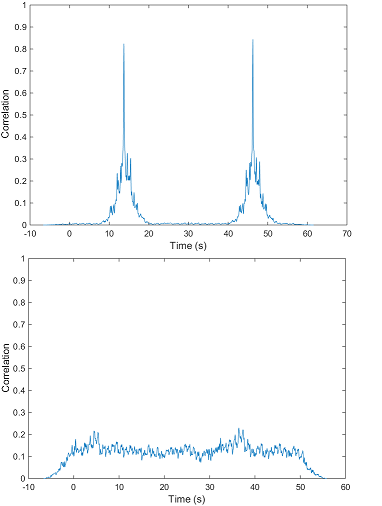
\includegraphics[width=\linewidth]{corr.png}
\caption{Geometric mean of correlation functions for when sample is present twice (above) and sample is absent (below)}
\label{fig1}
\end{figure}

\subsubsection{Pitch-shifting \& Time-stretching}
The assumption that the sample is neither time-stretched nor pitch-shifted is not true for the majority of cases {\color{red}(can you provide dataset statistics supporting this?)}. Pitch-shifting is often required for the sample to match the tonality of the song, and time-stretching is often required to adjust for tempo differences between sample and song.

%Pitch-shifting is a very common effect applied to samples before being used by artists in their own composition. It refers to the process of changing the pitch of the original sample up or down. 
In case of pitch-shifting, the sample templates $W_\mathrm{o}$ will no longer be valid templates since the frequency axis of the spectral content will be scaled by the pitch-shift factor. In order to account for pitch-shifting, we construct new sets of spectral templates by scaling the frequency axis of the templates with a number of hypothesized pitch-shift factors and create an extended $W_\mathrm{o}$ matrix. Now, a partially fixed NMF will be able to extract activations corresponding to each set of pitch-shifted templates and these may be compared to the activations from the original sample. {\color{red}wait, didn't you say you run an NMF per pitch? Is this still true? Also, give details about pitch shifting resolution and range}

%\subsubsection{Time-stretching}

%Time-stretching is another common effect used in sampling. Artists most often change the speed of the sample in order to match their own song's tempo. 
When the sample is time-stretched, the activations from the song will be similarly stretched and cross-correlation can no longer be used since the activation patterns stretched or compressed where the sample is present.
%
In such a scenario, DTW can be used to align the activations $H_\mathrm{o}$ with the activations $H_\mathrm{s}$ at a start frame $f$ in the song for each pitch-shift factor. A distance matrix is constructed using the pair-wise cosine distance between the $K$ dimensional activations. {\color{red}cosine distance is correct, right?}
\begin{figure}[t]
\centering
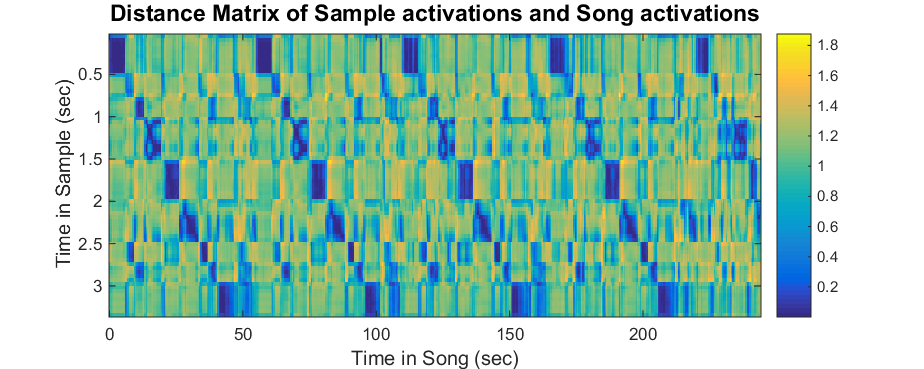
\includegraphics[width=\linewidth]{distmat.png}
\caption{Distance matrix computed between activations in the case where a sample is looped}
\label{fig2}
\end{figure}

This problem is now a subsequence search for the sample activations $H_\mathrm{o}$ within the series of activations corresponding to the sample templates in the song, $H_\mathrm{s}$. We compute the cost matrix using DTW. The cost matrix is initialized by accumulating the distance matrix along the direction of sample only. The accumulated cost of alignment is an indicator of whether a sample is present at a particular frame in time or not. {\color{red}what about the multiple nmfs? This has to be made clearer! Also, the explanation is not clear: direction of the sample only etc... rewrite the paragraph in context of the previous one, describe hte last row of the cost matrix etc}

\subsubsection{Activation Normalization}
Proper normalization of the activation function is essential for accurate sample detection, however, there is no ``correct'' way to do this as the level (or even its presence) of the sample in the query song is unknown. The relative activation levels between the $K$ templates of one set should remain identical, though. Thus, each set of activations is normalized by the absolute maximum across all the $K$ activations across time, preserving the relative activation strengths for the spectral templates of the sample:
%
\begin{equation}
H_{normalized} = \frac{H}{max(H^{k}_{t}: k\in[1,K], \forall N )}.
\end{equation}

Note that to account for pitch-shifting, there are $n$ sets of activations, where $n$ is the number of hypothesized pitch-shift factors. This normalization is applied to each of the $n$ sets of activations. 
{\color{red}Why would you use $n$ if the number of blocks is $N$. Introduce this variable earlier when you talk about pitch shifts and choose wisely.}

\subsubsection{Pitch Candidate Selection}
From the set of pitch-shifted activation functions, the candidate with the most likely pitch-shift factor has to be inferred. For each set of activations corresponding to the different pitch-shifted templates, the DTW cost matrix is computed. The most likely pitch candidate will be the one with the global minimum cost lower than that of all other candidates. All subsequent computations are based on the activation matrix of the selected candidate; the results for all other pitch-shifted templates are discarded.

\subsection{Feature Extraction}
The DTW cost matrix and properties of the extracted path can be used to indicate the presence of a sample in the query song. \figref{fig3} shows an example of a cost matrix with a looped sample. The low cost parallel blue paths indicate the presence of the sample. The last row of the matrix, containing the alignment path cost normalized by the length of the path, will be referred to as \textit{DTW cost function}. Local minima in the DTW cost function indicate potential sample end points.
%To detect whether a sample is present in a song, DTW costs are computed for alignment paths backtracking from all end frames in the song and normalized by the length of the path. This mapping for every end frame in the song to the DTW cost for the path ending at that frame is called the DTW cost function. Figure \ref{fig3} shows an example of this mapping. Ideally, the end frame where the sample ends will be a local or global minimum in the function.

\begin{figure}[t]
\centering
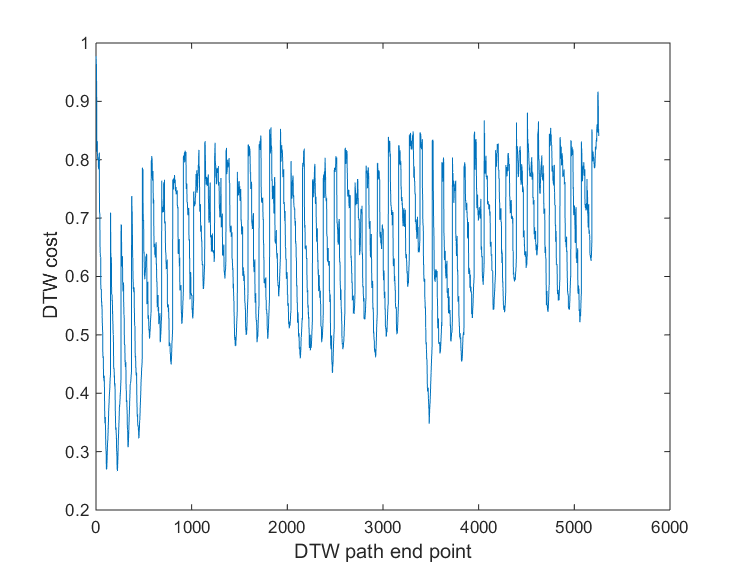
\includegraphics[width=\linewidth]{DTWcost.png}
\caption{DTW cost function; Minima indicate the end of the sample}
\label{fig3}
\end{figure}

Using an absolute threshold on the DTW cost function to detect a sample is not meaningful because a low alignment cost in one song might not be a low cost in another song. The mixing ratio of different samples in different songs will be different. Some might occur in a section with no other sources while others might be heavily overlaid with other sounds, leading to varying strength in activations across different song and sample pairs. Backtracking the DTW paths from all possible end points to their corresponding start location results in a set of unique start locations for each song and sample pair. Every unique start location is a candidate for a sample being present. Note that each unique start location can have multiple paths/end points. \figref{fig4} shows one example of this function.
The following features are extracted from this data. {\color{red}would it make sense to add more explanation as to why the designed features make sense?}

%Another feature obtained from the DTW is the location in the song at which an alignment path starts. Intuitively, given that a sample is present, the DTW backtracking path for end frames in the neighborhood of the exact location where the sample ends would also, after some DTW steps, merge into the optimal alignment path. Therefore, mapping the end points to the start points, we would observe a constant start point value for end points in the neighborhood of the location of the sample. This mapping is called the DTW path start function. Figure \ref{fig4} shows one example of this function. A flat step in this function refers to ending frames that map to the same start point in the song after DTW.

\begin{figure}[t]
\centering
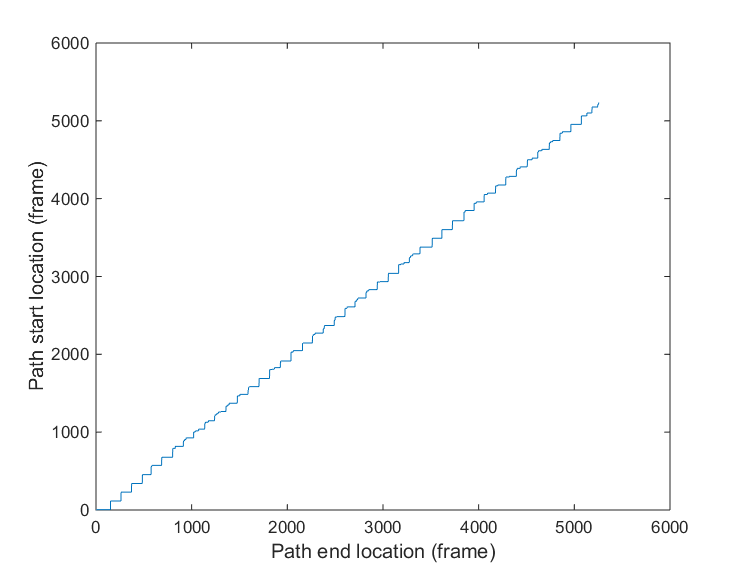
\includegraphics[width=\linewidth]{DTWpath.png}
\caption{DTW path start function; Longer steps indicate sample}
\label{fig4}
\end{figure}

%A valid assumption for each step in this function is that the local minimum of the DTW cost function should be considered as a candidate for sample detection. Hence for each song and sample pair, each unique start location in the DTW path start function is a candidate for classification and we extract the following features from the two aforementioned mappings as well as the DTW paths that were computed.

\subsubsection{Cost-based Features}
From the multiple path end points of each start location, the following three features are extracted: 
\begin{inparaenum}[(i)]
    \item   the minimum DTW cost across all end points,
    \item   the average DTW cost across all end points, and
    \item   the standard deviation of the DTW cost across all end points.
\end{inparaenum}
%We extract the local minimum of the DTW cost for each end point corresponding to the unique start location. Along with the minimum, we also compute the mean and standard deviation of the cost over the set of points that map to the current step. The costs are normalized by the DTW path length.

\subsubsection{Path-based Features}
The properties of the DTW alignment path should be meaningful for detecting the presence of the sample.  For example, the tempo of the sample should stay roughly constant, meaning that the slope of the path stays constant as well. Thus, the idealized path is computed by drawing a line from start point to end point. 
Overall, the following features are extracted:
\begin{inparaenum}[(i)]
    \item   the absolute length of the minimum cost path normalized by the sample length,
    \item   the slope of the minimum cost path, 
    \item   the average perpendicular deviation of the minimum cost path from the idealized path, normalized by the length of the path,
    \item   the average slope across all end point paths, 
    \item   {\color{red}it seems I have lost one feature!!!},
    \item   the average perpendicular deviation from the idealized path across all end point paths, normalized by the length of the paths,
    \item   the standard deviation of the perpendicular deviation from the idealized path across all end point paths, normalized by the length of the path, and
    \item   the number of end points for this unique start location.
\end{inparaenum}
%After extracting the local minimum DTW cost, we also extract the length and slope of the path for the minimum cost. In addition, we compute the mean deviation of the path's slope from a straight line. In this discretized space, the deviation is computed using euclidean geometry. The final features used are the length, slope and slope deviation of the minimum cost path, mean and standard deviation of path slopes within the step, and mean and standard deviations of all path lengths within the step.

%In addition, we use the length of the step in the DTW path start function corresponding to the current unique start location. This gives us a 11-dimensional feature space.

% \begin{enumerate}
% \item DTW cost: Local minimum in the DTW cost function.
% \item Slope deviation: Value at the index of minimum cost.
% \item Length of path for minimum cost.% Normalized by length of sample.
% \item Slope of path for minimum cost.
% \item Length of step in the DTW path start function corresponding to the current start location. %Normalized by length of the sample.
% \item Mean of the local cost for the current step.
% \item Standard deviation of the local cost for the current step.
% \end{enumerate}

% The DTW is also used to compute a feature we define as `slope deviation'. The slope deviation is another path feature which computes the deviation of the path from the average slope of that path normalized by the path length. This is computed using the perpendicular euclidean distance of every point in the path from the line joining the start and end points that that path.


\subsection{Classification}
\label{class}
Each unique start location is now represented by an 11-dimensional feature vector, which is a data point that can be used as the input to a binary classifier for detecting whether a sample is present or not.
%Given the set of features extracted for each unique start location, the task at hand is a simple binary classification. The definition of an instance or a data point $x$ in our case is: Every unique start location in the DTW path start function. The classifier needs to decide whether a sample is present at the location denoted by $x$.

A random forest classifier with an ensemble of 200 decision trees was chosen for this task \cite{breiman2001random}. The number of features chosen for each decision split is 4. The output is a probability of the data point belonging to each class.

% \begin{algorithm}
% \begin{enumerate}
% \item Compute the magnitude spectrogram of the original sample, $X_o$ and the song, $X_s$. 
% \item Compute the template $B_o$ and the activations $G_o$ from the sample spectrogram $X_o$ using NMF. The rank $k$ may be set based on the signal.
% \item Apply NMF on the song spectrogram $X_s$, but this time, make use of the templates $B_o$ in addition to other mixture templates while computing the NMF. This is called partially-fixed NMF.
% \item Correlate the activations $G_s$ corresponding to $B_o$ for the song spectrogram $X_s$ with the originally computed activations for the original sample $G_o$. In the ideal case, a correctly detected sample would mean that both the activations have a very high correlation at the position of occurrence as compared to other lags in time.
% \item Currently, return a positive match if peaks in the correlation function are greater than $0.6$. Figures \ref{fig1} and \ref{fig2} show the geometric means of correlations between 6 activations for the sample and the song, one for a true positive and one for a true negative.
% \end{enumerate}
% \caption{{\bf Non-negative Matrix Factorization-based Sample Detection} \label{Algorithm3}}
% \end{algorithm}

\section{Evaluation}
\label{eval}

\subsection{Dataset}
A dataset was compiled for this task using data from whosampled.com.\footnote{www.whosampled.com, last accessed: 1/22/2017} Whosampled.com is a website that aggregates information about songs that sample or cover other songs. The audio was downloaded using web services from streaming websites such as Youtube or Dailymotion.

80 samples were selected according to the following criteria:
\begin{inparaenum}[(i)]
    \item   the original songs are from influential artists like James Brown, Stevie Wonder, Michael Jackson and have been sampled multiple times, 
    \item   {\color{red}add more criteria (genres, length, etc.)}
\end{inparaenum}

    The songs that used these samples are in most cases from the genres Hip-Hop, Pop, and Rap. The samples in this dataset cover several variations of sampling such as: one-shot samples of musical snippets or voice samples, looped drums, and looped melodies. The longest sample is 25 seconds, the shortest is half a second and the average length of the samples is 4.5 seconds. The total number of sampling instances is 876. {\color{red}add info about pitch shifting and time-stretching. Also, would a plot with a distribution or something like that make sense?}
The overall dataset contains 80 pairs of original song and sampling song.

The following annotations were added manually with the software Sonic Visualizer \cite{SonicVisualiser}:
\begin{inparaenum}[(i)]
    \item   start and end time in seconds of the sample in the original song,
    \item   start time in seconds of the sample in the sampling song, and
    \item   pitch shift factor of the sample in the sampling song.
\end{inparaenum}
%For each original song, the start and end time of the segment that was sampled is manually annotated. In songs that used a sample, all start locations of the sample are annotated.
%%For each annotated sample, in the corresponding song that sampled it, all start locations of the sample are annotated. 
%All annotation is done using Sonic Visualizer \cite{SonicVisualiser}. In addition, the pitch-shift factor of the sample in the song are annotated.

These annotations plus additional meta-data including the song names, identifiers, and URLs for obtaining the audio have been made available publicly in an online repository.\footnote{www.github.com/placeholder\_repo}

\subsection{Experiments}
\label{exp}
For each of the 80 samples in our dataset, there are 79 songs in which the sample does not occur. We randomly pick {\color{red}(let's avoid the word sample here...)} 9 songs from these 79 songs; in combination with the one query song that includes the sample this results in 10 query songs for each sample, resulting in an overall number of query songs of $80\cdot10 = 800$ for the $80$ samples.
%In our experiments, we chose 10 songs for each of the samples in our dataset to detect sampling. Of the 10, the sample is only present in one song and the remaining 9 songs are randomly sampled from the set of songs that don't contain the sample. This gives us $80\times10 = 800$ sample-song pairs.

This overall set is split into a training set of 50 samples/500 queries and a test set of 30 samples/300 queries.
%To evaluate the classifier, the first 50 samples from dataset were chosen as the training set. Further, problematic samples were identified where there were no diagonals observed in the distance matrix. These were pruned from the subset. Section \ref{disc} will discuss these problematic samples. Experiments are carried out using both: the full training set and the pruned training set.

In order to allow using the ground truth data for training, one additional step of interaction is necessary: all unique start points have to be labeled as `0' or `1' based on whether a sample is present. %In order to achieve this without having to manually tag each unique start point, the ground truth of the time instants of where sample is present are used. 
More specifically, the start points associated with minimum DTW cost within a 1 second window of the ground truth annotation are labeled `1' and the rest are labeled `0'. %In some instances there were multiple start points within the tolerance window. To break these ties, instead of choosing the closest start location, the location that had the minimum cost DTW path was labeled `1' and the rest are labeled `0'. The reason for doing this is that, upon observation, it was found that some of these candidates were false positives with high DTW costs and we would like to train the classifier with less noisy data.

For the test set, any positive detection of the sample within a 1 second tolerance window of the ground truth annotation will be regarded as True Positive. Every positive detection outside of this tolerance window and for queries not containing the sample will be regarded as False Positive.
%For testing, the remaining 30 samples are used. For each of the 300 sample-song pairs, features are extracted and the predictions are obtained for each candidate sample location. For the sample-song pairs that contain the sample, the ground truth annotations are obtained and any positive detection within a 1 second tolerance window is classified as a true positive. 
If multiple positive detections are obtained in the tolerance window, all but the closest detection are classified as False Positives. {\color{red}wait. is this necessary? can't we just merge them and count them as one TP???}
%The remaining positive detections are also false positives. For sample-song pairs that don't contain the sample, any positive detections are obviously false positives. 
We report False Positive Rate, Precision, Recall, and F-measure for the sample location detection. We refer to these as \textit{Micro}-accuracy measures as they take into account the sample location and the number of occurrences.

The \textit{Macro}-accuracy measures, on the other hand, report the song-level sample detection results and indicate whether a sample is present in a song or not regardless of position and number of occurrences. The same measures False Positive Rate, Precision, Recall, and F-measure are reported, but the sample detection is evaluated per song rather than per sample instance.
%In addition to the micro-accuracy measures, we also report the song-level sample detection precision, recall and f-measure for a binary classifier for classifying whether a song contains a given sample or not. We refer to these as macro-accuracy measures. 
In summary, using both the Macro and Micro-level accuracy metrics we are able to report the performance of the method in two scenarios: First, detecting whether a sample is present in a song, and second, detecting where in a song and how often a given sample is present.

\section{Results}
{\color{red} I think we should just remove E2. Then we just combine results and discussion.}
The tables \ref{results} report the training accuracy as well as the testing accuracy for our classifier. For reference:
\begin{itemize}
\item E1: All $50 \times 10$ sample-song pairs are used to train the classifier.
\item E2: Some samples are pruned from the training set to remove cases where NMF activations fail to align. 12 samples are removed. Hence, $38 \times 10$ sample-song pairs are used to train the classifier.
\end{itemize}

\begin{table}[t]
\centering
\begin{tabular}{l|c|c|c|c|}
\cline{2-5}
                                & \multicolumn{2}{c|}{E1} & \multicolumn{2}{c|}{E2} \\ \cline{2-5} 
                                & Micro      & Macro      & Micro      & Macro      \\ \hline
\multicolumn{1}{|l|}{Precision} & 79.07\%    & 71.43\%    & 73.05\%    & 69.57\%    \\ \hline
\multicolumn{1}{|l|}{Recall}    & 35.29\%    & 50.00\%    & 35.64\%    & 53.33\%    \\ \hline
\multicolumn{1}{|l|}{F-measure} & 48.80\%    & 58.82\%    & 47.91\%    & 60.38\%    \\ \hline
\multicolumn{1}{|l|}{Fp-rate}   & 0.04\%     & 2.22\%     & 0.05\%     & 2.59\%     \\ \hline
\end{tabular}
\caption{Results for song-level macro accuracy and sample location-level micro accuracy measures}
\label{results}
\end{table}


\section{Discussion}
\label{disc}

Based on the results presented, it is clear that this method is somewhat effective at detecting the presence of sampling in a set of song with high precision and a very low false-positive rate. The low recall of the method can be attributed to the highly imbalanced nature of the problem. The testing dataset has 289 instances of sampling against around 74,000 instances that aren't locations of sampling. Similarly, the training set is also skewed in its distribution of positive and negative classes. We observed that recall could be improved by balancing the training data by undersampling the negative class instances but it led to a drastic decrease in the precision and f-measure. 

Another probably reason for the low recall is that the method isn't completely accurate when it comes to picking candidates. It misses out on approximately 8\% of sampling instances during the feature extraction stage. Furthermore, upon observation of some training examples, it was found that, the DTW cost function did not have a minimum at respective sample locations. While our classifier isn't trained to rely heavily on DTW cost alone but also on the alignment paths, we did observe that, in these problematic cases, the distance matrix would not contain clear alignment paths. This could lead to the problematic cases being misclassified as negatives, resulting in a low recall.

Absence of clear alignment paths stem from incorrect modeling of the fixed sample templates in the song NMF step, and/or due to the distance measure chosen. While the use of correlation makes sense because it emphasizes similarity in a sequence of values, there could still be a better distance measure for this particular use-case.

The problematic cases that we came across were not very straightforward cases of sampling. These samples were sparse drum loops, very short samples, very quiet in the mix, and some had other DSP effects applied to them. As mentioned in Section \ref{exp}, we conducted experiments with and without these problematic cases in the training data. Interestingly, removing these examples from the training data led to a slight decrease in the performance. A possible explanation for the drop in precision after removing these problematic cases could be that some representative negative song-sample pairs were also removed from the training set leading to more false-positives.
% \section{Discussion}
% \label{dis}

% While the algorithm discussed here seems simple and effective in solving the problem, there were several interesting nuances in the topic that were overlooked in previous work by Dittmar et al, as well as our initial implementation of the algorithm. This section will discuss some of these in detail.

% \subsection{DTW computation}

% In the current state, the distance matrix is computed using a correlation distance across the rank of the activation matrices. This kind of distance measure, however, doesn't account for any sparseness which is very likely in the NMF output. Distances between elements that are 0 shouldn't affect the overall distance as much as distances where the activations are higher and more similar. A new distance measure might be required to take into account this asymmetry in activation distances.

% \subsection{Normalization}

% The topic of normalization is one of the biggest issues that we faced and are still facing while devising this algorithm. The first step where normalization begins to affect the results is the normalization of the activations. Without normalizing the activations, the scale of the two sets of activations might be very different and any distance computation will be meaningless. Therefore, we currently normalize the activation with the maximum value in the activations for all templates. This makes sense against normalizing with the maximum per template because we want to preserve relative activations across the whole rank.

% The features that we use for the classification also need to be normalized appropriately in order to develop a generalized model. In the current state, the costs are normalized by the alignment path length, the length of the steps in the DTW path start function is normalized by the length of the sample in frames, the slope deviation is also normalized by the path length. While the choice of the alignment path for normalization makes sense, incorporating the time stretch factor, could be another approach to normalization.

% The discussion about NMF rank selection may also fall under the topic of normalization. If the parameters for the rank may be set correctly then it is possible that we can achieve better normalization of the final features across all samples and songs which will make a trained model more generalized.

% \subsection{Problematic Samples}

% While labelling the data before training or testing the classifier, it was observed that some samples weren't showing diagonal paths of low cost in the distance matrix unlike most of the other samples which were used for training and testing. Upon observation of these samples, it was noted that some of them were very short, quiet, were drum loops or had effects applied to them. These observations may or may not be the reason that the NMF activations distances aren't able to reveal the presence of the sample.

% Another possible explanation for this could be incorrectly annotated pitch-shift factors which will throw off the partially fixed NMF step of the algorithm. Further research needs to be done focusing on these samples to determine what is causing this.

\section{Future Work}

The method described in this paper is a promising step towards automatic sample detection, however, further research needs to be done in order to make this method practical. Since the broad algorithm involving NMF and DTW works for most cases, a systematic way to go about improving this method would we to investigate the problematic cases and drastically reduce false negatives.

As this problem is inherently unbalanced, a possible direction is to observe best practices for machine learning on imbalanced datasets. While we attempted undersampling, there are other techniques such as algorithmic modifications and cost-sensitive learning that may be employed to solve imbalanced classification problems \cite{lopez2013insight}.

Investigating custom distance measures for the DTW is another possible avenue to explore. Applying non-linearity to the NMF activations as a pre-processing step may also help in improving the features and eventually differentiating between an instance containing and sample and one that does not. While this should positively impact both, false positives and false negatives, false positives may also be reduced by post processing the classifier output, for example, by making sure a positive output is a local minimum in the DTW cost function.

\section{Conclusion}

%1. describe the algorithm in short again
%2. talk about dataset released
%3. talk about performance, high precision.
%4. Talk about future work

We introduce a method to automatically detect the presence of a sample in a set of songs based on NMF, to extract common activations for templates from the sample, and DTW, to align the set of activations obtained from the song and the sample. This method proposed is robust against common audio effects like pitch-shifting and time-stretching. We also present a new dataset of real-world samples and songs along with detailed annotations containing fine-grained annotations for exact time locations within the song. The method is evaluated against this dataset and we obtain 78\% precision in detecting the exact location of the sample and 74\% precision in song-level detection of a given sample. Some further directions of research have also been suggested which, supported by the new dataset, may be undertaken by the MIR community toward establishing a state-of-the-art in automatic sample detection.
% For bibtex users:
\newpage
\bibliography{ISMIRtemplate}

% For non bibtex users:
%\begin{thebibliography}{citations}
%
%\bibitem {Author:00}
%E. Author.
%``The Title of the Conference Paper,''
%{\it Proceedings of the International Symposium
%on Music Information Retrieval}, pp.~000--111, 2000.
%
%\bibitem{Someone:10}
%A. Someone, B. Someone, and C. Someone.
%``The Title of the Journal Paper,''
%{\it Journal of New Music Research},
%Vol.~A, No.~B, pp.~111--222, 2010.
%
%\bibitem{Someone:04} X. Someone and Y. Someone. {\it Title of the Book},
%    Editorial Acme, Porto, 2012.
%
%\end{thebibliography}

\end{document}
